\section{Exercise 1 - KKT conditions}
\subsection{Problem 1: KKT example 1}

\begin{equation}
    \min x_1+2x_2 s.t. 2-x_1^2-x_2^2 \geq 0, x_2 \geq 0
\end{equation}

\subsubsection{1a}
Given the constraint $c_1: 2-x_1^2-x_2^2 \geq 0$ the feasible area would be within a circle with radius $\sqrt2$.

From the constraint $c_2: x_2 \geq 0$ the resulting feasible are is within the upper half circle.

The objective function gradient is given by $\nabla f = \begin{bmatrix}
    1 & 2
\end{bmatrix}$

Can from these facts conclude that the optimal point would be in $x = (-\sqrt2,0)$. Because from this point there is no direction vector to move along which has a negative dot product with the gradient, and stays in the feasible set $\Omega$.

\subsubsection{1b}
Lagrangian:

\begin{subequations}
    \begin{align}
    \mathcal{L}(x,\lambda) = f(x) - \sum_{i \in \mathcal{E} \cup \mathcal{I}}\lambda_ic_i(x) \\        
    \mathcal{L}(x,\lambda) = x_1 + 2x_2 - \lambda_1 (2-x_1^2-x_2^2) - \lambda_2 x_2
\end{align}
\end{subequations}
KKT conditions:

\begin{subequations}
    \begin{align}
        \nabla_x\mathcal{L}(x^*,\lambda^*) = 0 \\
        c_1(x_1^*,x_2^*) \geq 0 \\ 
        c_2(x_1^*,x_2^*) \geq 0 \\ 
        \lambda_i^* \geq 0 , \forall i \in \mathcal{I} \\ 
        \lambda_i^*c_i(x^*) = 0 , \forall i \in \mathcal{I}
    \end{align}
\end{subequations}

\begin{subequations}
    \begin{align}
        \frac{\partial \mathcal{L}}{\partial x_1} = 1+2\lambda_1 x_1^* = 0\\ 
        \lambda_1 = -\frac{1}{2x_1^*} \\ 
        \frac{\partial \mathcal{L}}{\partial x_2} = 2 + 2\lambda_1 x_2^* - \lambda_2 = 0 \\ 
        \lambda_2 = 2\lambda_1 x_2^* + 2 \\ 
        \text{Inserting the optimal point to find lambda:} \\ 
        \lambda_1^* = -\frac{1}{-2\sqrt2} = \frac{1}{2\sqrt2} \\ 
        \lambda_2^* = \frac{1}{\sqrt2}*0+2 = 2 \\ 
        \lambda_1^* c_1(x^*) = \frac{1}{2\sqrt2} * (2-2) = 0 \\ 
        \lambda_2^* c_2(x^*) = 2*0 = 0
    \end{align}
\end{subequations}

As we see,the KKT conditions are satisfied.

%Solving for $\lambda$

%\begin{subequations}
%    \begin{align}
%        2 - (-\frac{1}{2\lambda_1})^2 - (\frac{\lambda_2-2}{2\lambda_1})^2 \geq 0 \\ 
%        \frac{\lambda_2 - 2}{2\lambda_1} \geq 0
%    \end{align}
%\end{subequations}

\subsubsection{1c}
Gradient of constraints and objective function at the solution:

\begin{subequations}
    \begin{align}
        \nabla f = \begin{bmatrix}
            1 & 2
        \end{bmatrix} \\ 
        \nabla c_1 = \begin{bmatrix}
            2\sqrt{2} & 0
        \end{bmatrix} \\ 
        \nabla c_2 = \begin{bmatrix}
            0 & 1
        \end{bmatrix}
    \end{align}
\end{subequations}

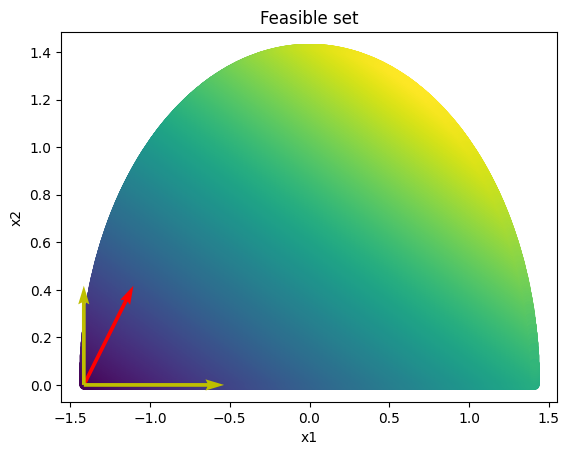
\includegraphics[width=8.0cm]{../.././images/1c.png}

\subsubsection{1d}
The lagrange coefficients for inequality constraints need to be positive such that the inequality dosent get flipped by multiplying a negative scalar. By following this, it ensures that lagrangian function is optimal.

\subsubsection{1e}
The given constraints are convex, because for any set of points in the feasible set, we can draw a line which stays within the set region.
The objective function is linear, which means it is also convex.
Thus, this optimization problem is convex.

\subsection{Problem 2: KKT example 2}
\subsubsection{1a}

\begin{subequations}
    \begin{align}
        \min 2x_1+x_2 s.t. x_1^2+x_2^2-2=0 \\ 
        \mathcal{L}(x,\lambda) = 2x_1+x_2 - \lambda (x_1^2+x_2^2-2) \\ 
        \nabla \mathcal{L} = \begin{bmatrix}
            2-2\lambda x_1 & 1-2\lambda x_2
        \end{bmatrix} \\ 
        2-2\lambda^* x_1^* = 0 => x_1^* = \frac{1}{\lambda^*} \\ 
        1-2\lambda^* x_2^* = 0 => x_2^* = \frac{1}{2\lambda^*} \\ 
        \lambda^* c(x^*) = 0 => \lambda^*(-2+\frac{1}{(\lambda^*)^2}+\frac{1}{4(\lambda^*)^2}) = 0 \\ 
        -2\lambda + \frac{1}{\lambda} + \frac{1}{4\lambda} = 0 => (\lambda^*)^2 = \frac{5}{8} \\ 
        \lambda^* = \pm \sqrt{\frac{5}{8}} \\ 
        x_1^* = \pm 2\sqrt{\frac{2}{5}} \\ 
        x_2^* = \pm \sqrt{\frac{2}{5}}
    \end{align}
\end{subequations}

\subsubsection{2b}
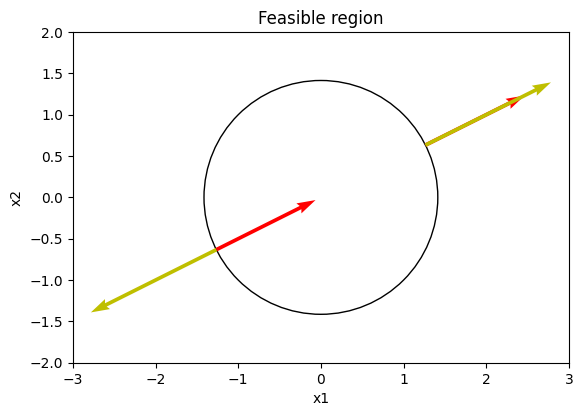
\includegraphics[width=8.0cm]{../.././images/2b}

\subsubsection{2c}
The value of the lagrangian multiplier is $\lambda = \pm\sqrt{\frac{5}{8}}$ which makes sense with KKT because the constraint is an equality condition.


\subsubsection{2d}
Left KKT point is a local solutions because the neighbourhood of points have a bigger f value, while for rightmost point, there is no neighbourhood of points with bigger f value.

\subsubsection{2e}
\begin{subequations}
    \begin{align}
        \omega^T \nabla^2_{xx} \mathcal{L}(x^*,\lambda^*)\omega > 0 \\ 
        \nabla^2_{xx} \mathcal{L} = \begin{bmatrix}
            -2\lambda & 0 \\ 
            0 & -2\lambda 
        \end{bmatrix}
    \end{align}
\end{subequations}

Given the point where $\lambda = -\sqrt(\frac{5}{8})$, the matrix is positive definite, s.t. the requirment holds. $x^*$ is a strict local solution.
\subsubsection{2f}
The problem is not convex because the for two points in the feasible set , it cant be drawn a line where every point on the line is in the feasible set. Easier said, the feasible set is along the circlebow.

\subsection{Problem 3: Second-order conditions}
\begin{subequations}
    \begin{align}
        \min -2x_1+x_2 s.t.
        \left\{\begin{aligned}
            c_1:(1-x_1)^3-x_2 \geq 0 \\
            c_2:x_2 + \frac{1}{4}x_1^2 - 1 \geq 0
        \end{aligned}
        \right. 
    \end{align} 
\end{subequations}
The given optimal point is $x^* = (0,1)$

\subsubsection{3a}
\begin{subequations}
    \begin{align}
    \mathcal{A}(x^*) = {1,2} \\ 
    -3*(1-x_1)^2 = -3 \\ 
    \nabla c_1(x^*) = \begin{bmatrix}
        -3 & -1
    \end{bmatrix}^T \\ 
    \nabla c_2(x^*) = \begin{bmatrix}
        0 & 1
    \end{bmatrix}^T
\end{align}
\end{subequations}

Because the gradients of the constraints in active set $\mathcal{A}$ are lineary independent, LICQ holds at the optimal point.

\subsubsection{3b}
\begin{subequations}
    \begin{align}
        \mathcal{L}(x,\lambda) = -2x_1+x_2-\lambda_1((1-x_1)^3-x_2)-\lambda_2(x_2+\frac{1}{4}x_1^2-1) \\ 
        \nabla \mathcal{L} = \begin{bmatrix}
            -2+3\lambda_1(1-x_1)^2-\frac{1}{2}\lambda_2 x_1 & 1+\lambda_1-\lambda_2 
        \end{bmatrix} \\ 
        -2+3\lambda_1= 0 => \lambda_1 = \frac{2}{3} \\ 
            \lambda_2 = 1 + \lambda_1 = \frac{5}{3}
    \end{align}
\end{subequations}

Which are both positive, so KKT conditions are fullfilled.

\subsubsection{3c}

\begin{subequations}
    \begin{align}
    \nabla c_1(x^*) = \begin{bmatrix}
        -3 & -1
    \end{bmatrix}^T \\ 
    \nabla c_2(x^*) = \begin{bmatrix}
        0 & 1
    \end{bmatrix}^T \\ 
    \mathcal{F} = d^T\nabla c_i(x) \geq 0 \\ 
    \begin{bmatrix}
        d_1 & d_2
    \end{bmatrix}\begin{bmatrix}
        -3 \\ 
        -1
    \end{bmatrix} = -3d_1-d_2 \geq 0 \\ 
    \begin{bmatrix}
        d_1 & d_2
    \end{bmatrix}\begin{bmatrix}
        0 \\ 
        1
    \end{bmatrix} = d_2 \geq 0 \\ 
    d_1 \leq -\frac{d_2}{3} \\ 
    \omega_2 = 0 \\ 
    \omega_1 = 0 \\ 
    \omega = \begin{bmatrix}
        0 \\ 
        0
    \end{bmatrix}
\end{align}
\end{subequations}
The critical cone only contains zero vector
\subsubsection{3d}
Because the 2. order inequality are for vectors excluding zero-vector, and we only have zero-vector in critical cone, we can conclude $x^*$ to be strict local solution.

\subsection{Problem 4: Find optimizers}

\begin{subequations}
    \begin{align}
    \min -x_1x_2 \\ 
    c_1: x_1^2+x_2^2 = 1
\end{align}
\end{subequations}

\begin{subequations}
\begin{align}
    \mathcal{L} = -x_1x_2 - \lambda (1-x_1^2-x_2^2) \\ 
    \nabla \mathcal{L} = \begin{bmatrix}
        -x_2+2\lambda x_1 & -x_1+2\lambda x_2 
        \end{bmatrix} \\ 
\end{align}
\end{subequations}









